\section{Sheared Flow Results}

The axial Mach number for these sheared flow validation cases were taken to be,

\begin{align}
    M_x = M_0 \left( 1 - \bar{r}_{Shankar} \right)^{ \frac{1}{7}}
    \label{eqn:cylindricalShear} \\
\end{align}

where $\bar{r}_{Shankar} = \frac{r_{min}}{r_{max}-r_{min}} = \frac{r_{min}}{b}$ 

Since the radius is non-dimensionalized differently in \ref{Shankar1972}, the 
velocity profile defined as a function of $\bar{r}_{Shankar}$.


\begin{figure}[h!]
    \centering
    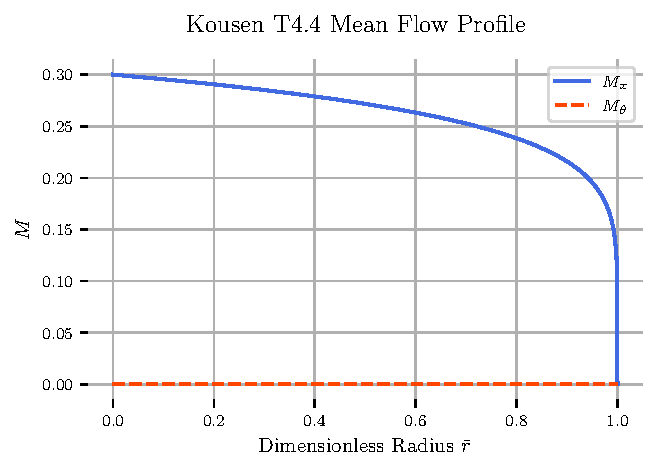
\includegraphics{/home/jeff-severino/SWIRL/CodeRun/04-plotReport/tex-outputs/KousenT2_mean_flow_profile.pdf}
    \caption{Mean mach number profile for the uniform flow in a lined cylinder}
    \label{fig:1}
\end{figure}

\begin{figure}[h!]
    \centering
    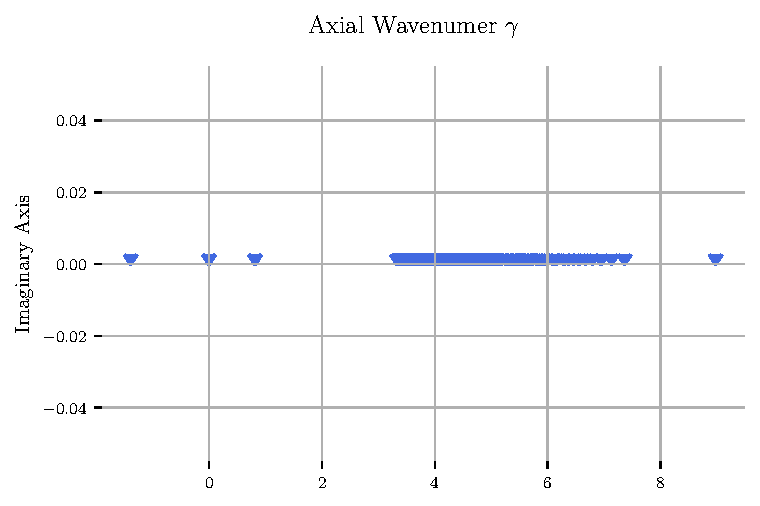
\includegraphics[width=\textwidth]{/home/jeff-severino/SWIRL/CodeRun/04-plotReport/tex-outputs/KousenT2_gam_nonconv_scatter_4thOrderApprox.pdf}
\end{figure}


